
\documentclass{report}
\usepackage[margin=0.5in]{geometry}
\usepackage[T1]{fontenc}
\usepackage{lmodern} % must be loaded with fontenc --- otherwise text will become bitmaps
\usepackage[british]{babel}
\usepackage{csquotes} % will automatically use quotes of the babel language
\usepackage{amssymb}
\usepackage{amsmath}
\usepackage{amsthm}
\usepackage{mathtools}
\usepackage{etoolbox}
\usepackage{tabularx}
\usepackage{booktabs}
\usepackage{listings}
\usepackage{color}
\usepackage[normalem]{ulem}
\usepackage[style=apa]{biblatex} % verbose or apa depending on cite style
\usepackage{xcolor}
\usepackage[
    colorlinks,
    linkcolor=blue,
    citecolor=blue,
    urlcolor=blue
]{hyperref}
\usepackage[capitalize]{cleveref} % use capitalization so that we do not need to worry about detecting beginnings of sentences, etc
\usepackage{import}
\usepackage[useregional]{datetime2}
\usepackage{titlesec}
\usepackage{physics}
\usepackage{float} % for H option in table
\usepackage{parskip} % remove indentation on new paragraphs
\usepackage{caption}
\usepackage[export]{adjustbox} % allow max width
\usepackage{graphbox} % allow align=t in \includegraphics to make them work better in minipages if first item

\MakeOuterQuote{"}

\titleformat{\chapter}[display]{}{}{0pt}{\raggedright\normalfont\bfseries\huge\thechapter\hspace*{1em}}[] % for chapters created from metadata blocks
\titleformat{name=\chapter,numberless}[display]{}{}{0pt}{\raggedright\normalfont\bfseries\huge\phantom{\thechapter}\hspace*{1em}}[] % for unnumbered chapters, including the table of contents
\titlespacing{\chapter}{0pt}{2em}{1em}

\lstset{
	backgroundcolor=\color[rgb]{1,1,1},
	tabsize=4,
	rulecolor=,
	basicstyle=\ttfamily,
	upquote=true,
	aboveskip={1.5\baselineskip},
	columns=fixed,
	showstringspaces=false,
	extendedchars=true,
	breaklines=true,
	prebreak = \raisebox{0ex}[0ex][0ex]{\ensuremath{\hookleftarrow}},
	showtabs=false,
	showspaces=false,
	showstringspaces=false,
	identifierstyle=\ttfamily,
	keywordstyle=\color[rgb]{0,0,1},
	commentstyle=\color[rgb]{0.133,0.545,0.133},
	stringstyle=\color[rgb]{0.627,0.126,0.941},
	aboveskip=0pt,
	literate={£}{{\textsterling{}}}1 % allow £ sign within listings
}

\newcommand{\noncolouredtableofcontents}{
	\begingroup
	\hypersetup{hidelinks}
	\tableofcontents
	\endgroup
}

\ifcsundef{thematicbreak}{\newcommand{\thematicbreak}{\par\bigskip\noindent\hrulefill\par\bigskip}}{}

\theoremstyle{definition}
\ifcsundef{definition}{\newtheorem{definition}{Definition}[section]}{}

\theoremstyle{plain}
\ifcsundef{theorem}{\newtheorem{theorem}{Theorem}[section]}{}
\ifcsundef{lemma}{\newtheorem{lemma}[theorem]{Lemma}}{}
\ifcsundef{corollary}{\newtheorem{corollary}{Corollary}[theorem]}{}

\theoremstyle{definition}
\ifcsundef{definition}{\newtheorem{definition}{Definition}[section]}{}
\ifcsundef{example}{\newtheorem{example}{Example}[section]}{}

\theoremstyle{remark}
\ifcsundef{assumption}{\newtheorem*{assumption}{Assumption}}{}
\ifcsundef{proof}{\newtheorem*{proof}{Proof}}{}
\ifcsundef{exercise}{\newtheorem{exercise}{Exercise}[section]}{}
\ifcsundef{problem}{\newtheorem{problem}{Problem}[section]}{}
\ifcsundef{question}{\newtheorem{question}{Question}[section]}{}
\ifcsundef{tip}{\newtheorem*{tip}{Tip}}{}
\ifcsundef{solution}{\newtheorem*{solution}{Solution}}{}
\ifcsundef{note}{\newtheorem{note}{Note}[section]}{}
\ifcsundef{derivation}{\newtheorem{derivation}{Derivation}[section]}{}
\ifcsundef{axiom}{\newtheorem{axiom}{Axiom}[section]}{}
\ifcsundef{conjecture}{\newtheorem{conjecture}{Conjecture}[section]}{}
\ifcsundef{hypothesis}{\newtheorem{hypothesis}{Hypothesis}[section]}{}
\ifcsundef{proposition}{\newtheorem{proposition}{Proposition}[section]}{}

\ifcsundef{remark}{\newtheorem*{remark}{Remark}}{} % notes are numbered but remarks are not

\renewcommand{\qedsymbol}{$\blacksquare$} % closed black square for proof environments

\renewcommand\thesection{\arabic{section}}

\numberwithin{equation}{section}
\numberwithin{figure}{section}
\numberwithin{table}{section}

\providecommand{\tightlist}{%
  \setlength{\itemsep}{0pt}\setlength{\parskip}{0pt}}
  
% fix parskip within minipage
\setlength{\parskip}{\medskipamount}
\makeatletter
\newcommand{\@minipagerestore}{\setlength{\parskip}{\medskipamount}}
\newcommand{\mathcolorbox}[2]{\colorbox{#1}{$\displaystyle #2$}}
\makeatother

\newcommand*{\matr}[1]{\mathbfit{#1}}
\newcommand*{\tran}{^{\mkern-1.5mu\mathsf{T}}}
\newcommand*{\conj}[1]{\overline{#1}}
\newcommand*{\hermconj}{^{\mathsf{H}}}

\usepackage[inline]{enumitem}

\usepackage{tikz}
\usepackage[tikz]{ocgx2}
\usetikzlibrary{tikzmark, fit, calc, positioning,arrows.meta}

\bibliography{bib.bib}

\begin{document}

\setcounter{secnumdepth}{3}

\section{Preliminaries: Constituent and Dependency Trees}
Let \(w = \qty(w_{1}, \ldots, w_{L})\) be a sentence.

A \textit{constituent tree} is a rooted tree whose leaves are the words \(\qty(w_{i})_{i=1}^{N}\) and internal nodes are constituents.

A \textit{constituent} is a triple \(\qty(\tikzmarknode{const-label}{Z}, \tikzmarknode{const-yield}{\mathcal{Y}}, \tikzmarknode{const-head}{h})\) containing, respectively, its label, yield, and lexical head which satisfy some constraints\footnote{A leaf node can be modelled as a constituent whose yield contains only its head. For every constituent \(\qty(Z, \mathcal{Y}, h)\) with children \(\qty{\qty(A_{k}, \mathcal{X}_{k}, m_{k})}\), \begin{enumerate*} \item \(\mathcal{Y} = \bigcup_{k=1}^{K} \mathcal{X}_{k}\), and \item there is a unique \(k\) such that \(h = m_{k}\). \end{enumerate*}}.

A constituent is \tikzmarknode{disc-text}{\textit{discontinuous}} if its yield is not contiguous.

A \textit{dependency tree} is a rooted tree spanning the words in the sentence \(\qty(w_{i})_{i=1}^{N}\). Each edge is labelled and connects a parent word (head) to a child word (dependency).

\textcite{fernandez2015parsing} show that under quite general conditions\footnote{The constituent trees must be unaryless.}, constituent trees are isomorphic to dependency trees in which the edges contain information about constituent labels and attachment order.

\begin{figure}[H]
    \centering
    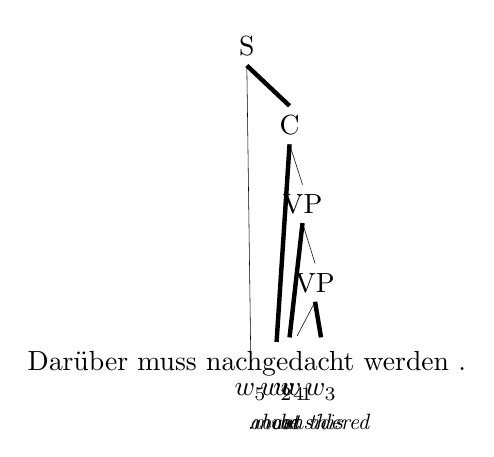
\begin{tikzpicture}[remember picture]
        \node[inner sep=0, text depth=0] (w) {\subnode[inner sep=0]{s-yld}{\subnode[inner sep=0]{c-yld}{\subnode[inner sep=0]{vptop-left}{\subnode[inner sep=0]{vpbot-left}{\subnode[inner sep=2pt]{w1}{Darüber}}} \subnode[inner sep=2.5pt]{w2}{muss} \subnode[inner sep=0]{vptop-right}{\subnode[inner sep=0]{vpbot-right}{\subnode[inner sep=1.5pt]{w3}{nachgedacht}} \subnode[inner sep=1.5pt]{w4}{werden}}} \subnode[inner sep=2.5pt]{w5}{.}}};
    
        \foreach \n/\english in {1/about this,2/must,3/considered,4/be,5/.} \node[below=1ex of {w\n |- w.south}, inner sep=0, align=center] {\(w_{\n}\) \\[0ex] \scalebox{0.8}{\textit{\english}}};
        
        % \coordinate (s) at ({barycentric cs:w1=1,w2=1,w3=1,w4=1} |- {barycentric cs:w=1,vroot=4});
        
        \node[switch ocg=const-s] (vroot) at ($(w) + (0, 4cm)$)  {S};
        \node[switch ocg=const-c] (s) at ({barycentric cs:w1=1,w2=3,w3=1,w4=1} |- {barycentric cs:w=1,vroot=3}) {C};
        \node[switch ocg=const-vptop] (vp1) at ({barycentric cs:w1=1,w3=1,w4=1} |- {barycentric cs:w=2,vroot=2}) {VP};
        \node[switch ocg=const-vpbot] (vp2) at ({barycentric cs:w1=1,w3=3} |- {barycentric cs:w=3,vroot=1}) {VP};
    
        \draw[very thin] (vroot.south) -- (w5.north);
        \draw[ultra thick] (vroot.south) -- (s.north);
        \draw[ultra thick] (s.south) -- (w2.north);
        \draw[very thin] (s.south) -- (vp1.north);
        \draw[ultra thick] (vp1.south) -- (w4.north);
        \draw[very thin] (vp1.south) -- (vp2.north);
        \draw[very thin] (vp2.south) -- (w1.north);
        \draw[ultra thick] (vp2.south) -- (w3.north);
    \end{tikzpicture}
    \caption{Example of a discontinuous constituent tree for the German sentence \textit{"Darüber muss nachgedacht werden."} ("this must be considered."). Bold lines indicate head words.} \label{fig-c-tree}
\end{figure}

\begin{tikzpicture}[remember picture, overlay]
    % vptop
    \begin{scope}[ocg={ref=const-vptop, status=invisible, opts={radiobtngrp=const}}]
        \node[draw, fit=(vp1), fill=red, inner sep=0, opacity=0.5] {};
        \node[draw, fit=(vptop-right), fill=green, inner sep=0, minimum height=1em, opacity=0.5] {};
        \node[draw, fit=(vptop-left), fill=green, inner sep=0, minimum height=1em, opacity=0.5] {};
        \node[draw, fit=(w4), fill=cyan, inner sep=0, minimum height=1em, opacity=0.5] {};
        \draw[ultra thick, cyan] (vp1.south) -- (w4.north);

        % highlight in definition
        \node[draw, fit=(const-label), fill=red, inner sep=0, opacity=0.5] {};
        \node[draw, fit=(const-yield), fill=green, inner sep=0, opacity=0.5] {};
        \node[draw, fit=(const-head), fill=cyan, inner sep=0, opacity=0.5] {};
        \node[draw, fit=(disc-text), fill=yellow, inner sep=0, opacity=0.5] {};
    \end{scope}

    % vpbot
    \begin{scope}[ocg={ref=const-vpbot, status=invisible, opts={radiobtngrp=const}}]
        \node[draw, fit=(vp2), fill=red, inner sep=0, opacity=0.5] {};
        \node[draw, fit=(vpbot-right), fill=green, inner sep=0, minimum height=1em, opacity=0.5] {};
        \node[draw, fit=(vpbot-left), fill=green, inner sep=0, minimum height=1em, opacity=0.5] {};
        \node[draw, fit=(w3), fill=cyan, inner sep=0, minimum height=1em, opacity=0.5] {};
        \draw[ultra thick, cyan] (vp2.south) -- (w3.north);

        % highlight in definition
        \node[draw, fit=(const-label), fill=red, inner sep=0, opacity=0.5] {};
        \node[draw, fit=(const-yield), fill=green, inner sep=0, opacity=0.5] {};
        \node[draw, fit=(const-head), fill=cyan, inner sep=0, opacity=0.5] {};
        \node[draw, fit=(disc-text), fill=yellow, inner sep=0, opacity=0.5] {};
    \end{scope}

    % c-yld
    \begin{scope}[ocg={ref=const-c, status=invisible, opts={radiobtngrp=const}}]
        \node[draw, fit=(s), fill=red, inner sep=0, opacity=0.5] {};
        \node[draw, fit=(c-yld), fill=green, inner sep=0, minimum height=1em, opacity=0.5] {};
        \node[draw, fit=(w2), fill=cyan, inner sep=0, minimum height=1em, opacity=0.5] {};
        \draw[ultra thick, cyan] (s.south) -- (w2.north);

        % highlight in definition
        \node[draw, fit=(const-label), fill=red, inner sep=0, opacity=0.5] {};
        \node[draw, fit=(const-yield), fill=green, inner sep=0, opacity=0.5] {};
        \node[draw, fit=(const-head), fill=cyan, inner sep=0, opacity=0.5] {};
    \end{scope}

    % s-yld
    \begin{scope}[ocg={ref=const-s, status=invisible, opts={radiobtngrp=const}}]
        \node[draw, fit=(vroot), fill=red, inner sep=0, opacity=0.5] {};
        \node[draw, fit=(s-yld), fill=green, inner sep=0, minimum height=1em, opacity=0.5] {};
        \node[draw, fit=(w2), fill=cyan, inner sep=0, minimum height=1em, opacity=0.5] {};
        \draw[ultra thick, cyan] (vroot.south) -- (s.north);
        \draw[ultra thick, cyan] (s.south) -- (w2.north);
        
        % highlight in definition
        \node[draw, fit=(const-label), fill=red, inner sep=0, opacity=0.5] {};
        \node[draw, fit=(const-yield), fill=green, inner sep=0, opacity=0.5] {};
        \node[draw, fit=(const-head), fill=cyan, inner sep=0, opacity=0.5] {};
    \end{scope}
\end{tikzpicture}

\begin{figure}[H]
    \centering
    
\begin{tikzpicture}[remember picture]
        \node (w) at (0,0) {\subnode[inner sep=2pt]{wd1}{Darüber} \subnode[inner sep=2.5pt]{wd2}{muss} \subnode[inner sep=1.5pt]{wd3}{nachgedacht} \subnode[inner sep=1.5pt]{wd4}{werden} \subnode[inner sep=2.5pt]{wd5}{.}};

        % muss
        \draw[-Stealth] ($(wd2.north) + (2pt, 0)$) to [bend left=50] node [above, scale=0.5] {\(\mathrm{C}_{1}\)} ($(wd4.north) + (2pt, 0)$);
        \draw[-Stealth] ($(wd2.north) + (2pt, 0)$) to [bend left=80] node [above, scale=0.5] (s2) {\(\mathrm{S}_{2}\)} (wd5.north);

        % werden
        \draw[-Stealth] ($(wd4.north) - (2pt, 0)$) to [bend right=30] node [above, scale=0.5] {VP} ($(wd3.north) + (2pt, 0)$);

        % nachgedacht
        \draw[-Stealth] ($(wd3.north) - (2pt, 0)$) to [bend right=60] node [above, scale=0.5] {VP} (wd1.north);

        \node[scale=0.5] (root) at ({$(wd2) - (2pt, 0)$} |- s2) {\texttt{root}};
        \draw[-Stealth] (root.south) -- (root |- wd2.north);
    \end{tikzpicture}
    \caption{The dependency tree corresonding to the constituent tree in \cref{fig-c-tree}.}
\end{figure}

\section{Mathematical Model}
\begin{figure}[H]
    \centering
    
\begin{tikzpicture}[remember picture]
        \node (wdd) at (0,0) {\subnode[inner sep=0]{start}{\hspace{6em}} \subnode[inner sep=2pt]{wdd1}{Darüber} \subnode[inner sep=2.5pt]{wdd2}{muss} \subnode[inner sep=1.5pt]{wdd3}{nachgedacht} \subnode[inner sep=1.5pt]{wdd4}{werden} \subnode[inner sep=2.5pt]{wdd5}{.}};

        % lines and text
        % muss
        \draw[blue,thick,Stealth-] ($(wdd2.north) + (6pt, 0)$) to [bend left=50] node [black,above, scale=0.5] {\(\mathrm{C}_{1}\)} ($(wdd4.north) + (2pt, 0)$);
        \draw[blue,thick,Stealth-] ($(wdd2.north) + (3pt, 0)$) to [bend left=80] node [black,above, scale=0.5] (s2) {\(\mathrm{S}_{2}\)} (wdd5.north);

        % werden
        \draw[blue,thick,Stealth-] ($(wdd4.north) - (2pt, 0)$) to [bend right=30] node [black,above, scale=0.5] {VP} ($(wdd3.north) + (2pt, 0)$);

        % nachgedacht
        \draw[blue,thick,Stealth-] ($(wdd3.north) - (2pt, 0)$) to [bend right=60] node [black,above, scale=0.5] {VP} (wdd1.north);

        % root
        \node[black,scale=0.5] (root) at ({$(wdd2) - (2pt, 0)$} |- s2) {\texttt{root}};
        \draw[blue,thick,Stealth-] (root.south) -- (root |- wdd2.north);
        \foreach \i/\m in {1/{0/PAV},2/{0/VM,1/fin,2/ind,3/sing,4/pres},3/{0/V,1/part},4/{0/VA,1/inf},5/{0/\$.}}
        {
            \foreach \j/\k in \m
            {
                \node[scale=0.8,gray,inner sep=0] (pos\i\j) at ($({wdd\i.center |- wdd.south}) - (0, 1pt) - (0, 1.7ex * \j) $) {\k};
            }
        }

        \foreach \j/\t in {0/POS,1/morph.mood,2/morph.form,3/morph.number,4/morph.tense}
        {
            \node[scale=0.8,gray,inner sep=0,anchor=west] at (start.west |- pos2\j) {\texttt{\t}};
        }
    \end{tikzpicture}
\end{figure}

Given regressor \(w = \qty(w_{i})_{i=1}^{N}\), our goal is to model its dependency tree along with information like its part-of-speech (POS) and morphology.

Our parser will work from the bottom-up, so we will think of \textit{arcs} going from every child \(w_{i}\) to its parent \(w_{i}^{\mathrm{arc}}\).

Denote the regressand by \(y = \qty(y_{i})_{i=1}^{N}\) where \(y_{i} = \qty(w_{i}^{\mathrm{arc}}, w_{i}^{\mathrm{lab}}, w_{i}^{\mathrm{ord}}, w_{i}^{\mathrm{pos}}, w_{i}^{\mathrm{morph}})\). Define \(y_{<i} = \qty(y_{1}, \ldots, y_{i})\) for each \(i = 2, \ldots, N\) and \(y_{<1} = 0\).

\begin{assumption}
    For each \(i = 1, \ldots, N\), the random variables \(w_{i}^{\mathrm{lab}}, w_{i}^{\mathrm{ord}}, w_{i}^{\mathrm{pos}}\) and \(w_{i}^{\mathrm{morph}}\) are mutually independent conditional on \(w_{i}^{\mathrm{arc}}\), \(w\) and \(y_{<i}\).\footnote{If \(w_{i}^{\mathrm{morph}}\) is a vector, assume every component is mutually independent with each other and with \(w_{i}^{\mathrm{lab}}, w_{i}^{\mathrm{ord}}, w_{i}^{\mathrm{pos}}\) conditional on \(w_{i}^{\mathrm{arc}}, y_{<i}, w\)}.
\end{assumption}

We can decompose the conditional probability of \(y\) given \(w\):
\begin{align}
    p(y \mid w) &= \prod_{i=1}^{N} p(y_{i} \mid y_{<i}, w) \\
                &= \boxed{\prod_{i=1}^{N} p(w_{i}^{\mathrm{arc}} \mid y_{<i}, w) p(w_{i}^{\mathrm{lab}} \mid w_{i}^{\mathrm{arc}}, y_{<i}, w) p(w_{i}^{\mathrm{ord}} \mid w_{i}^{\mathrm{arc}}, y_{<i}, w) p(w_{i}^{\mathrm{pos}} \mid w_{i}^{\mathrm{arc}}, y_{<i}, w) p(w_{i}^{\mathrm{morph}} \mid w_{i}^{\mathrm{arc}}, y_{<i}, w).}
\end{align}


\section{Encoder-Decoder Setup}
Let \(N = \qty{1, \ldots, n}\) be an index set. Given an input sentence \(w = \qty(w_{i})_{i=1}^{N}\) we generate a sequence of \textit{embeddings} \(\boldsymbol{\omega} = \qty(\boldsymbol{\omega}_{i})_{i=1}^{N}\) where
\[
    \boldsymbol{\omega}_{i} = \mathbf{WordEmbed}(w_{i}) \oplus \mathbf{CharEmbed}(w_{i}) \oplus \mathbf{BertEmbed}(w_{i}).
\]

Character-level embeddings are implemented via a CNN á la \textcite{chiu2016named}. BERT embeddings are finetuned from a BERT model pre-trained on German text by \textcite{bert-base-german-cased}.

\textbf{Encoder}: feed embeddings through a multi-layer bi-directional LSTM with skip-connections and dropout:
\[
    \vb{e} = \qty(\vb{e}_{i})_{i = 0, \ldots, n} = \mathbf{BiLSTM}(\boldsymbol{\omega})
\]

\textbf{Decoder}: feed embeddings through a single-layer uni-directional LSTM with dropout:
\[
    \vb{d} = \qty(\vb{d}_{i})_{i = 1, \ldots, n} = \mathbf{LSTM}(\boldsymbol{\omega})
\]

\section{Bi-affine Attention Mechanism}
We feed \(\vb{e}\) and \(\vb{d}\) through MLPs to produce sequences \((\vb{e}^{\mathrm{arc}}, \vb{d}^{\mathrm{arc}})\) of dimension-reduced vectors. These are fed into a bi-affine layer which produces latent features \(\vb{v}^{\mathrm{arc}}\) that are then fed into an attention layer, resulting in logits corresponding to strength of an arc.
\begin{align}
    \vb{e}^{\mathrm{arc}} &= \mathbf{MLP}_{\mathrm{enc}}^{\mathrm{arc}}(\vb{e}); \qquad \qquad \vb{d}^{\mathrm{arc}} = \mathbf{MLP}_{\mathrm{dec}}^{\mathrm{arc}}(\vb{d}) \\
    \vb{v}^{\mathrm{arc}}_{i,j} &= \mathbf{BiAff}^{\mathrm{arc}}(\vb{e}^{\mathrm{arc}}_{i}, \vb{d}^{\mathrm{arc}}_{j}) \\
    &\coloneqq {\vb{e}^{\mathrm{arc}}_{i}}\tran \mathbf{U}_{\text{h-d}}^{\mathrm{arc}} \vb{d}_{i}^{\mathrm{arc}}  + \mathcolorbox{yellow}{
            {\vb{e}_{i}^{\mathrm{arc}}}\tran \mathbf{U}_{\text{h-h}}^{\mathrm{arc}} \vb{e}_{i}^{\mathrm{arc}}
            + {\vb{d}_{i}^{\mathrm{arc}}}\tran \mathbf{U}_{\text{d-d}}^{\mathrm{arc}} \vb{d}_{i}^{\mathrm{arc}}
        } \\
        &\phantom{\coloneqq}\  + U_{\text{h}}^{\mathrm{arc}} \vb{e}_{i}^{\mathrm{arc}}
        + U_{\text{d}}^{\mathrm{arc}} \vb{d}_{i}^{\mathrm{arc}}
        + \vb{u}_{\text{bias}}^{\mathrm{arc}} \\
        s_{i,j}^{\mathrm{arc}} &= \mathcolorbox{yellow}{{\vb{u}_{\text{agg}}^{\mathrm{arc}}} \tran \mathrm{tanh}(\vb{v}_{i,j}^{\mathrm{arc}})}
\end{align}

Fixing dependency \(j\), the vector \(\mathbf{softmax}(\vb{s}_{:, j})\) can be interpreted as an estimated probability distribution over potential heads.
\[
    \hat{p}^{\mathrm{arc}}(w_{i} \mid y_{<j}, w) = \mathbf{softmax}(\vb{s}_{:,j}^{\mathrm{arc}})_{i}.
\]

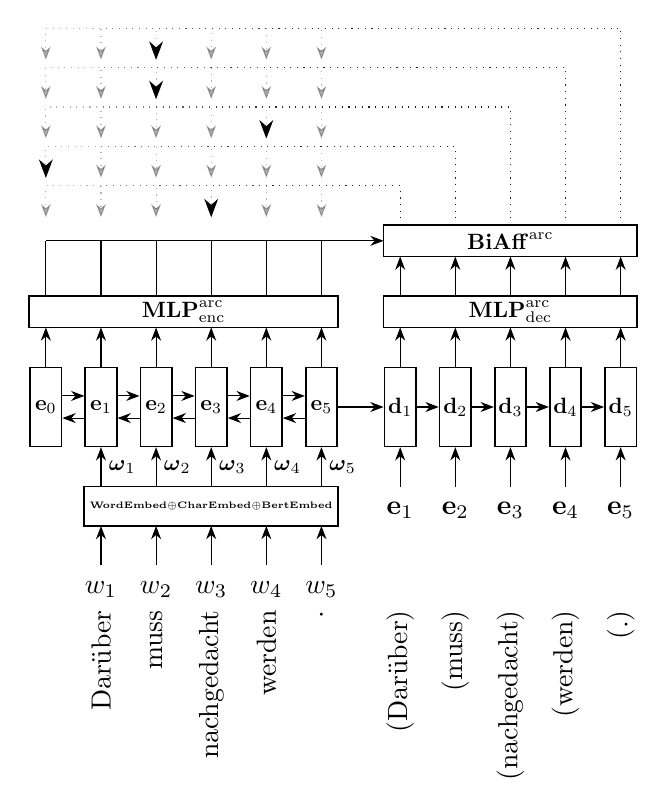
\begin{tikzpicture}
    \foreach \word / \n / \s in {/0/, Darüber/1/\(w_{1}\), muss/2/\(w_{2}\), nachgedacht/3/\(w_{3}\), werden/4/\(w_{4}\), ./5/\(w_{5}\)}
    {
        \node[
            shape=rectangle,
            inner sep=0pt,
            fill=none,
            text=black,
            anchor=north
        ] (wd\n) at (0.7 * \n, 0) {\rotatebox{90}{\word}};
        \node[
            name=w\n,
            above=0.2cm of wd\n,
            text depth=0,
            text height=1em,
            inner sep=0
        ] {\s};
    }

    \coordinate[above=0.5cm of w1.north west] (embedbl) {};
    \coordinate[above=1cm of w5.north east] (embedtr) {};
    \draw[semithick] (embedbl) rectangle (embedtr) node [pos=0.5,scale=0.68] {\(\scriptscriptstyle\mathbf{WordEmbed} \oplus \mathbf{CharEmbed} \oplus \mathbf{BertEmbed}\)};

    \foreach \n in {0,1,2,3,4,5}
    {
        \node[
            above = 0.5cm of {w\n |-embedtr},
            draw,
            rectangle,
            semithick,
            inner sep=0,
            minimum width=0.4cm,
            minimum height=1cm,
            label={[scale=0.8]center:$\vb{e}_{\n}$}
        ] (e\n) {};
    }

    \foreach \n in {1,2,3,4,5}
    {
        \draw[-Stealth] (w\n.north) -- (w\n|-embedbl);
        \draw[-Stealth] (w\n |- embedtr) -- (e\n.south) node[midway, right, scale=0.8] {\(\boldsymbol{\omega}_{\n}\)};
    }

    \foreach \n/\m in {0/1,1/2,2/3,3/4,4/5}
    {
        \draw[-Stealth] ($(e\n.east) + (0, 4pt)$) -- ($(e\m.west) + (0, 4pt)$) {};
        \draw[Stealth-] ($(e\n.east) - (0, 4pt)$) -- ($(e\m.west) - (0, 4pt)$) {};
    }

    \foreach \n/\j in {0/1,1/2,2/3,3/4,4/5}{
        \node[
            draw,
            rectangle,
            semithick,
            inner sep=0,
            minimum width=0.4cm,
            minimum height=1cm,
            label={[scale=0.8]center:$\vb{d}_{\j}$}
        ] (d\j) at ($(e5) + (1 + 0.7 * \n, 0)$) {};
    }

    \draw[-Stealth] (e5) -- (d1);

    \foreach \n/\m in {1/2,2/3,3/4,4/5}
    {
        \draw[-Stealth] (d\n) -- (d\m) {};
    }
    \foreach \word/\j in {Darüber/1,muss/2,nachgedacht/3,werden/4,./5}
    {
        \node[
            anchor=north,
            text depth=0,
            text height=1em,
            inner sep=0
        ] (ecopy\j) at (d\j |- embedtr.north) {$\vb{e}_{\j}$} edge[-Stealth] (d\j);
        \node[
            shape=rectangle,
            inner sep=0pt,
            fill=none,
            text=black,
            anchor=north
        ] at (wd\j.north -| ecopy\j) {\rotatebox{90}{(\word)}};
    }

    \coordinate[above=0.5cm of e0.north west] (mlpencbl) {};
    \coordinate[above=0.9cm of e5.north east] (mlpenctr) {};
    \draw[semithick] (mlpencbl) rectangle (mlpenctr) node [pos=0.5,scale=0.8] {\(\mathbf{MLP}_{\mathrm{enc}}^{\mathrm{arc}}\)};

    \coordinate[above=0.5cm of d1.north west] (mlpdecbl) {};
    \coordinate[above=0.9cm of d5.north east] (mlpdectr) {};
    \draw[semithick] (mlpdecbl) rectangle (mlpdectr) node [pos=0.5,scale=0.8] {\(\mathbf{MLP}_{\mathrm{dec}}^{\mathrm{arc}}\)};

    \foreach \i in {0,1,2,3,4,5}
    {
        \draw[-Stealth] (e\i.north) -- (e\i |- mlpencbl);
    }

    \coordinate[above=0.5cm of {mlpdecbl |- mlpdectr}] (biafbl) {};
    \coordinate[above=0.4cm of {biafbl -| mlpdectr}] (biaftr) {};
    \draw[semithick] (biafbl) rectangle (biaftr) node [pos=0.5,scale=0.8] (biaf) {\(\mathbf{BiAff}^{\mathrm{arc}}\)};
    \foreach \i in {0,1,2,3,4,5}
    {
        \draw (e\i.north |- mlpenctr) -- (e\i |- biaf);
    }
    \draw[-Stealth] (e0.north |- biaf) -- (biaf.west -| biafbl);

    \foreach \j in {1,2,3,4,5}
    {
        \draw[-Stealth] (d\j.north) -- (d\j |- mlpdecbl);
        \draw[-Stealth] (d\j |- mlpdectr) -- (d\j |- biafbl);
        \coordinate (p\j) at ($(biaftr) + (0, 0.5cm * \j)$);
        \coordinate (q\j) at ($(biaftr) + (0, 0.5cm * \j) - (0, 0.4cm)$);
    }
    \foreach \j in {1,2,3,4,5}
    {
        \foreach \i in {0,1,2,3,4,5} {
            \draw[opacity=0.3, dotted,arrows=-Stealth] (biaftr -| d\j) -- (p\j -| d\j) -- (p\j -| e\i) -- (q\j -| e\i);
        }
    }
    \foreach \j\i in {1/3,2/0,3/4,4/2,5/2}
    {
        \path[tips,black,thick,dotted,arrows={-Stealth}] (p\j -| e\i) -- (q\j -| e\i);
    }
\end{tikzpicture}

\section{Bi-affine Classifier for Attachment Order, POS and Morphology}
Attachment order, POS and morphologies are predicted via a classification layer. We use a bi-affine classifier which allows us to model probabilities of classes \textit{conditional} on arcs, and thus use structural cues in addition to encoder/decoder states to better capture the complexity of the language. The encoder and decoder are \textit{shared} across the tasks.

For example suppose we would like to predict the part of speech \(c \in \mathcal{C}\) for word \(w_{j}\) conditional on its parent being \(w_{i}\).
\begin{align}
    \vb{e}^{\mathrm{pos}} &= \mathbf{MLP}_{\mathrm{enc}}^{\mathrm{pos}}(\vb{e}); \qquad \qquad \vb{d}^{\mathrm{pos}} = \mathbf{MLP}_{\mathrm{dec}}^{\mathrm{pos}}(\vb{d}) \\
    \vb{v}^{\mathrm{pos}}_{i,j} &= \mathbf{BiAff}^{\mathrm{pos}}(\vb{e}^{\mathrm{pos}}_{i}, \vb{d}^{\mathrm{pos}}_{j}) \\
    &\coloneqq {\vb{e}^{\mathrm{pos}}_{i}}\tran \mathbf{U}_{\text{h-d}}^{\mathrm{pos}} \vb{d}_{i}^{\mathrm{pos}}  + 
            {\vb{e}_{i}^{\mathrm{pos}}}\tran \mathbf{U}_{\text{h-h}}^{\mathrm{pos}} \vb{e}_{i}^{\mathrm{pos}}
            + {\vb{d}_{i}^{\mathrm{pos}}}\tran \mathbf{U}_{\text{d-d}}^{\mathrm{pos}} \vb{d}_{i}^{\mathrm{pos}}
         \\
        &\phantom{\coloneqq}\  + U_{\text{h}}^{\mathrm{pos}} \vb{e}_{i}^{\mathrm{pos}}
        + U_{\text{d}}^{\mathrm{pos}} \vb{d}_{i}^{\mathrm{pos}}
        + \vb{u}_{\text{bias}}^{\mathrm{pos}} \\
        \hat{p}^{\mathrm{pos}}(c \mid w_{i}; y_{<j}, w) &= \mathbf{softmax}(\vb{v}^{\mathrm{pos}}_{i,j})_{c}
\end{align}


\begin{figure}[H]
    \centering
    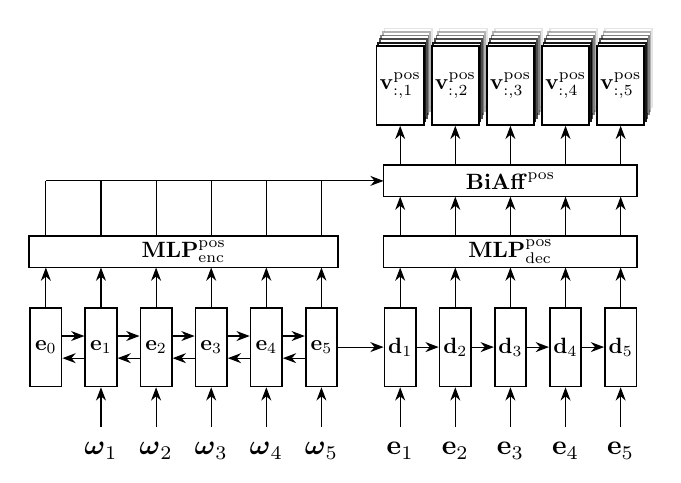
\begin{tikzpicture}
        \foreach \word / \n in {\texttt{root}/0, Darüber/1, muss/2, nachgedacht/3, werden/4, ./5}
        {
            \node[overlay,transparent,
                shape=rectangle,
                inner sep=0pt,
                fill=none,
                text=black,
                anchor=north
            ] (wd\n) at (0.7 * \n, 0) {\rotatebox{-90}{\word}};
            \node[overlay,transparent,
                name=w\n,
                above=0.2cm of wd\n,
                text depth=0,
                text height=1em,
                inner sep=0
            ] {$w_{\n}$};
        }

        \coordinate[above=0.5cm of w0.north west] (embedbl) {};
        \coordinate[above=1cm of w5.north east] (embedtr) {};
        \draw[overlay,transparent,semithick] (embedbl) rectangle (embedtr) node [pos=0.5,scale=0.8] {\(\mathbf{WordEmbed} \oplus \mathbf{CharEmbed} \oplus \mathbf{BertEmbed}\)};

        \foreach \n in {0,1,2,3,4,5}
        {
            \draw[overlay,transparent,-Stealth] (w\n.north) -- (w\n|-embedbl);
            \node[
                above = 0.5cm of {w\n |-embedtr},
                draw,
                rectangle,
                semithick,
                inner sep=0,
                minimum width=0.4cm,
                minimum height=1cm,
                label={[scale=0.8]center:$\vb{e}_{\n}$}
            ] (e\n) {};
            \draw[overlay,transparent,-Stealth] (w\n |- embedtr) -- (e\n.south);
        }

        \foreach \n/\m in {0/1,1/2,2/3,3/4,4/5}
        {
            \draw[-Stealth] ($(e\n.east) + (0, 4pt)$) -- ($(e\m.west) + (0, 4pt)$) {};
            \draw[Stealth-] ($(e\n.east) - (0, 4pt)$) -- ($(e\m.west) - (0, 4pt)$) {};
        }

        \foreach \n/\j in {0/1,1/2,2/3,3/4,4/5}{
            \node[
                draw,
                rectangle,
                semithick,
                inner sep=0,
                minimum width=0.4cm,
                minimum height=1cm,
                label={[scale=0.8]center:$\vb{d}_{\j}$}
            ] (d\j) at ($(e5) + (1 + 0.7 * \n, 0)$) {};
        }

        \draw[-Stealth] (e5) -- (d1);

        \foreach \n/\m in {1/2,2/3,3/4,4/5}
        {
            \draw[-Stealth] (d\n) -- (d\m) {};
        }
        \foreach \word/\j in {Darüber/1,muss/2,nachgedacht/3,werden/4,./5}
        {
            \node[
                anchor=north,
                text depth=0,
                text height=1em,
                inner sep=0
            ] (ecopy\j) at (d\j |- embedtr.north) {$\vb{e}_{\j}$} edge[-Stealth] (d\j);
            \node[overlay,transparent,
                shape=rectangle,
                inner sep=0pt,
                fill=none,
                text=black,
                anchor=north
            ] at (wd\j.north -| ecopy\j) {\rotatebox{-90}{(\word)}};
        }

        \foreach \i in {1,2,3,4,5}
        {
            \node[
                anchor=north,
                text depth=0,
                text height=1em,
                inner sep=0
            ] (omega\i) at (e\i |- embedtr.north) {$\boldsymbol{\omega}_{\i}$} edge[-Stealth] (e\i);
        }

        \coordinate[above=0.5cm of e0.north west] (mlpencbl) {};
        \coordinate[above=0.9cm of e5.north east] (mlpenctr) {};
        \draw[semithick] (mlpencbl) rectangle (mlpenctr) node [pos=0.5,scale=0.8] {\(\mathbf{MLP}_{\mathrm{enc}}^{\mathrm{pos}}\)};

        \coordinate[above=0.5cm of d1.north west] (mlpdecbl) {};
        \coordinate[above=0.9cm of d5.north east] (mlpdectr) {};
        \draw[semithick] (mlpdecbl) rectangle (mlpdectr) node [pos=0.5,scale=0.8] {\(\mathbf{MLP}_{\mathrm{dec}}^{\mathrm{pos}}\)};

        \foreach \i in {0,1,2,3,4,5}
        {
            \draw[-Stealth] (e\i.north) -- (e\i |- mlpencbl);
        }

        \coordinate[above=0.5cm of {mlpdecbl |- mlpdectr}] (biafbl) {};
        \coordinate[above=0.4cm of {biafbl -| mlpdectr}] (biaftr) {};
        \draw[semithick] (biafbl) rectangle (biaftr) node [pos=0.5,scale=0.8] (biaf) {\(\mathbf{BiAff}^{\mathrm{pos}}\)};
        \foreach \i in {0,1,2,3,4,5}
        {
            \draw (e\i.north |- mlpenctr) -- (e\i |- biaf);
        }
        \draw[-Stealth] (e0.north |- biaf) -- (biaf.west -| biafbl);

        \foreach \j in {1,2,3,4,5}
        {
            \draw[-Stealth] (d\j.north) -- (d\j |- mlpdecbl);
            \draw[-Stealth] (d\j |- mlpdectr) -- (d\j |- biafbl);
        }

        \foreach \j in {1,2,3,4,5}
        {
            \coordinate (start\j) at (d\j |- {$(biaftr) + (0, 0.5cm)$});
            \foreach \k/\o in {5/0.1,4/0.3,3/0.5,2/0.7,1/0.9}
                {
                    \node[
                        draw,
                        draw opacity=\o,
                        rectangle,
                        semithick,
                        inner sep=0,
                        minimum width=0.6cm,
                        minimum height=1cm,
                        anchor=south,
                        fill=white
                    ] (hello) at ($(start\j) + (0.02 * \k, 0.045 * \k)$) {};
                }
            \node[
                draw,
                anchor=south,
                rectangle,
                semithick,
                inner sep=0,
                minimum width=0.6cm,
                minimum height=1cm,
                fill=white,
                label={[scale=0.8]center:$\vb{v}^{\mathrm{pos}}_{:,\j}$},
            ] (posclass\j) at (start\j) {} edge[Stealth-] (d\j |- biaftr);
        }
    \end{tikzpicture}
\end{figure}

\printbibliography
\end{document}